\chapter{Projeto Conceitual do Produto}

\section{Características gerais}

A Estrutura Analítica do Projeto (EAP), conforme definida pelo PMBOK Guide – Sexta Edição \cite{pmbok2017}, consiste em uma decomposição hierárquica e orientada a entregas do escopo total do projeto. Sua função é organizar e subdividir o trabalho em partes menores e gerenciáveis, facilitando o planejamento, a execução eo controle das entregas do projeto.

A seguir, apresenta-se a EAP desenvolvida para o projeto \textit{Foguete d’Água com Base Automatizada}, estruturada com base em seis pacotes principais de trabalho, que refletem os pilares técnicos e gerenciais do projeto.

\subsection{Decomposição Inicial}

A decomposição do escopo do projeto resultou nos seguintes pacotes principais: Planejamento e Gerenciamento, Estruturas, Software, Hardware, Energia e Integração. A Figura \ref{fig_eap_unificado} apresenta o primeiro e o segundo níveis da EAP.

\begin{figure}[!h]
	\centering
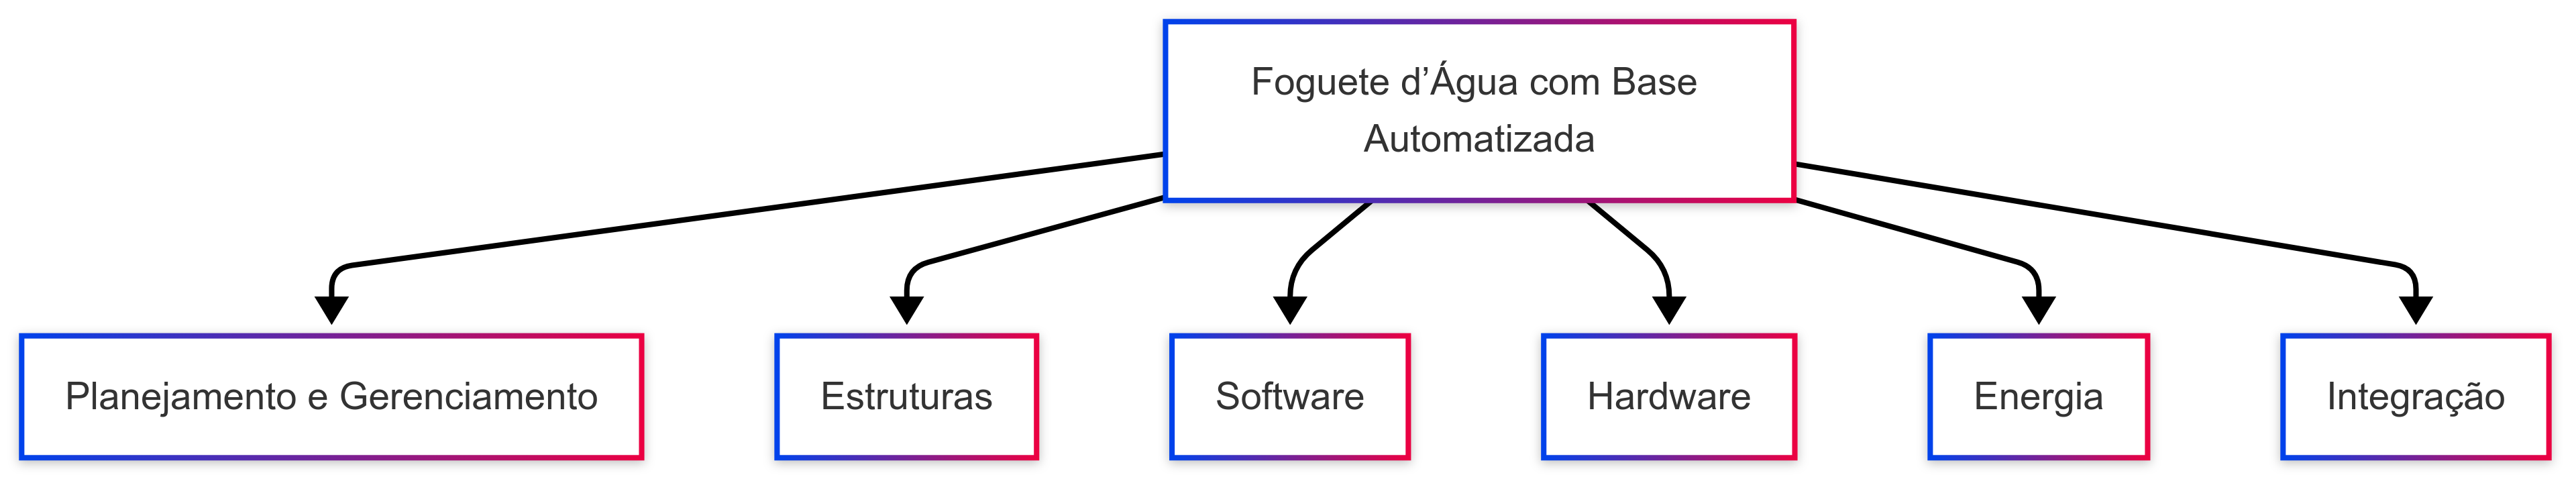
\includegraphics[width=15cm]{figuras/eap_unificado.png}
	\caption{EAP Geral}
	\label{fig_eap_unificado} 
\end{figure}

\subsection{Planejamento e Gerenciamento}

Este pacote de trabalho contempla os processos de iniciação, planejamento e monitoramento do projeto. Abrange a elaboração do Termo de Abertura do Projeto (TAP), a consolidação da EAP e dos cronogramas setoriais, o planejamento orçamentário, os relatórios de acompanhamento (planejado x realizado) e as atividades de encerramento, como eventos de avaliação SWOT, lições aprendidas e avaliação de desempenho da equipe, conforme a Figura \ref{fig_eap_planejamento}.

\begin{figure}[!h]
	\centering
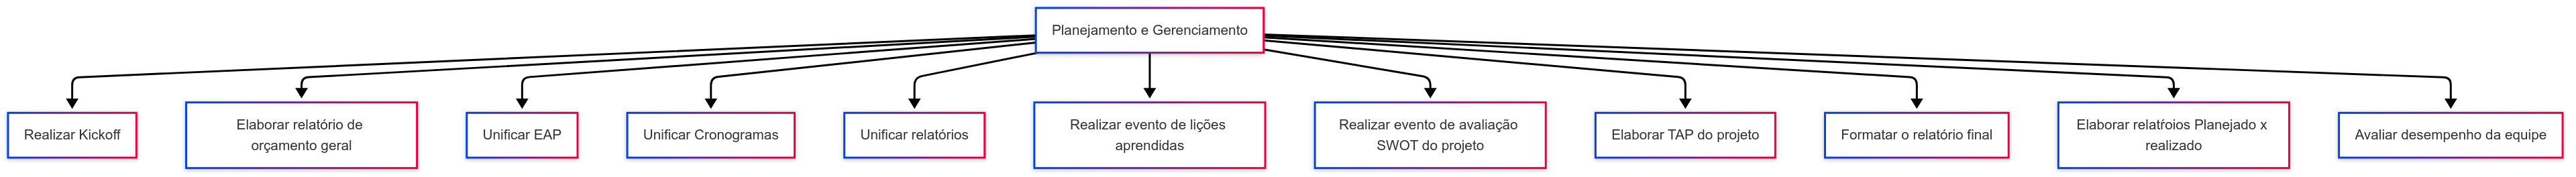
\includegraphics[width=15cm]{figuras/eap_planejamento.png}
	\caption{Pacote de Trabalho 1.1 – Planejamento e Gerenciamento}
	\label{fig_eap_planejamento} 
\end{figure}

\subsection{Estruturas}

Responsável pela modelagem e construção da fuselagem do foguete e da base física de lançamento. Este pacote inclui atividades como elaboração de desenhos técnicos em CAD, levantamento de materiais, montagem estrutural, e realização de experimentos e testes de integração estrutural. Também contempla a avaliação do desempenho de fornecedores, conforme ilustrado na Figura \ref{fig_eap_estruturas}.

\begin{figure}[!h]
	\centering
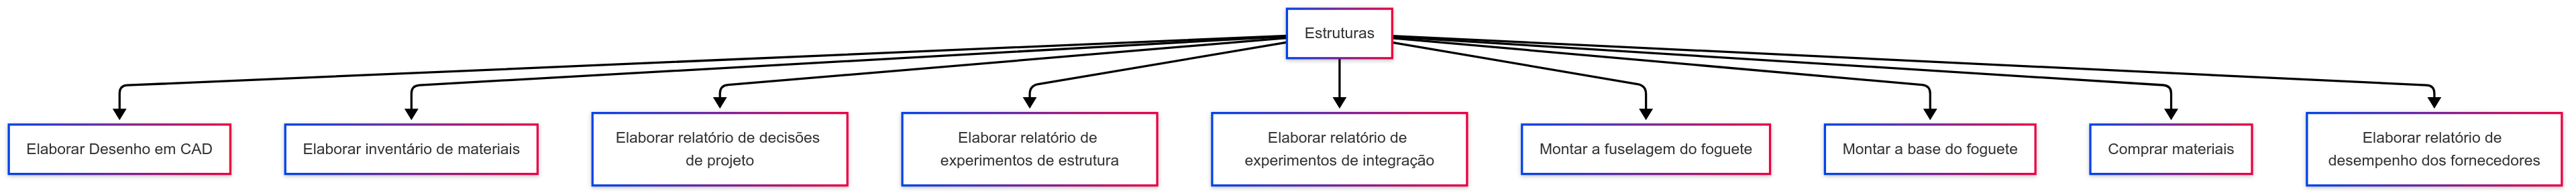
\includegraphics[width=15cm]{figuras/eap_estruturas.png}
	\caption{Pacote de Trabalho 1.2 – Estruturas}
	\label{fig_eap_estruturas} 
\end{figure}

\subsection{Software}

Este pacote compreende a elicitação de requisitos funcionais e não funcionais, a modelagem da arquitetura do sistema, a construção e testes de software. Inclui ainda a elaboração de diagramas (casos de uso, estados, BPMN), BACKLOG, DER, protótipos navegáveis e relatórios de testes de unidade e integração, conforme apresentado na Figura \ref{fig_eap_software}.


\begin{figure}[!h]
	\centering
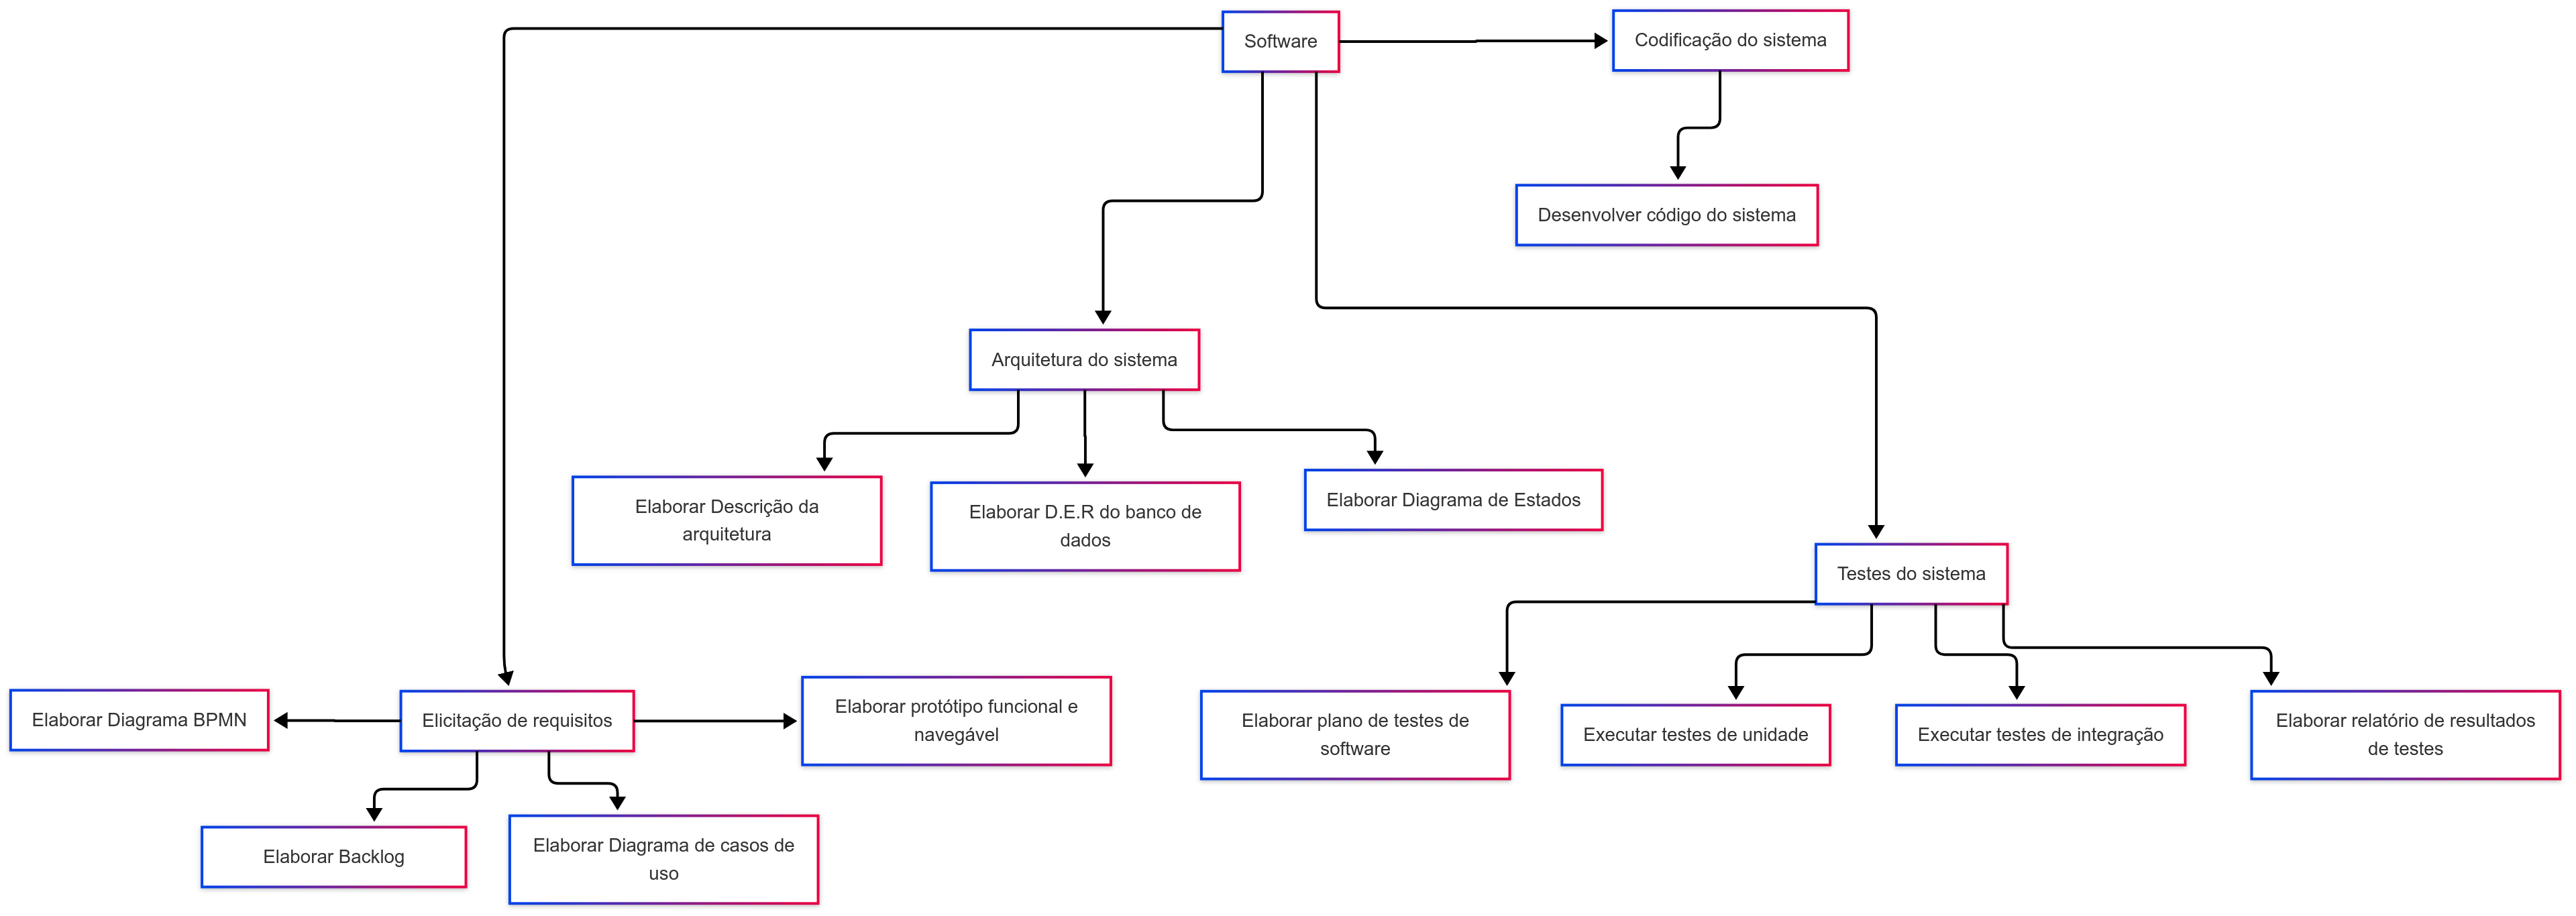
\includegraphics[width=15cm]{figuras/eap_software.png}
	\caption{Pacote de Trabalho 1.3 – Software}
	\label{fig_eap_software} 
\end{figure}

\subsection{Hardware}

Este pacote contempla a concepção eletrônica do sistema, incluindo a elaboração de diagramas de blocos e esquemáticos, a instalação de sensores e atuadores no foguete e na base de lançamento, além da realização de experimentos de hardware e de integração. Envolve também a documentação técnica e a avaliação do desempenho dos fornecedores, conforme Figura \ref{fig_eap_hardware}.


\begin{figure}[!h]
	\centering
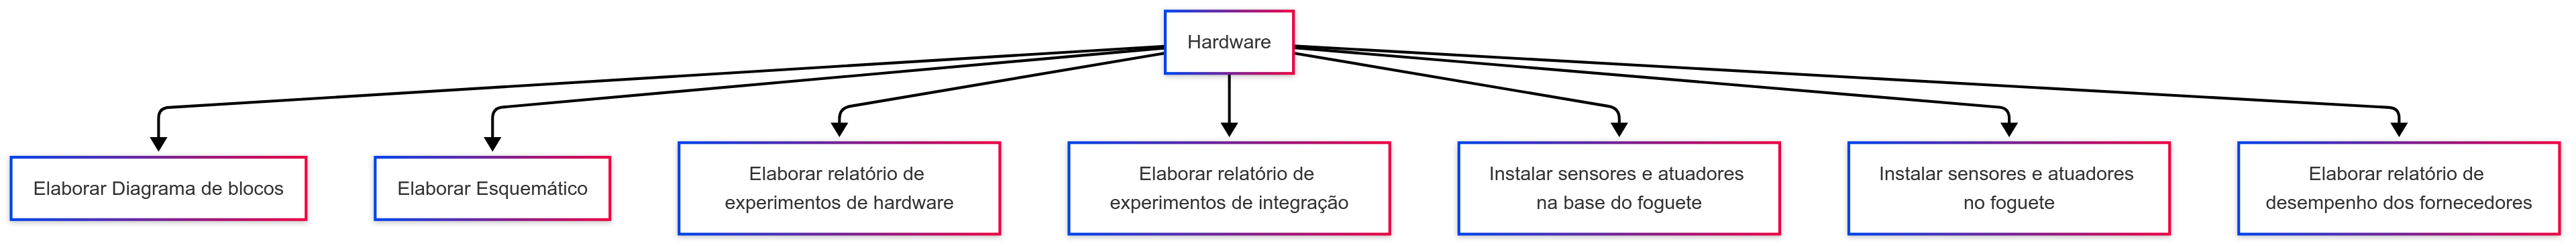
\includegraphics[width=15cm]{figuras/eap_hardware.png}
	\caption{Pacote de Trabalho 1.4 – Hardware}
	\label{fig_eap_hardware} 
\end{figure}

\subsection{Energia}

Foca na análise do consumo energético do sistema, na seleção e validação da fonte de alimentação e na condução de experimentos relacionados à autonomia e estabilidade energética. Assim como nas demais frentes técnicas, inclui relatório de desempenho dos fornecedores de componentes de energia, conforme Figura \ref{fig_eap_energia}.

\begin{figure}[!h]
	\centering
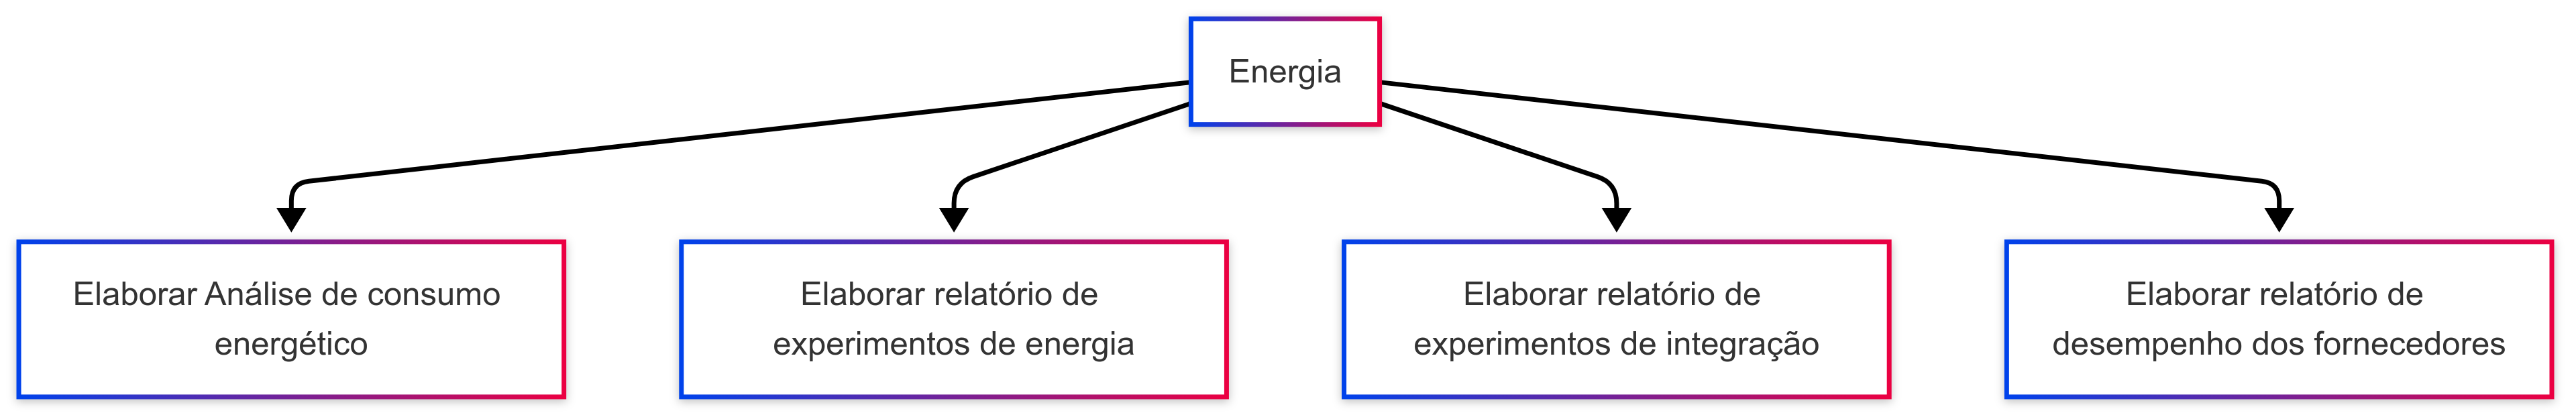
\includegraphics[width=15cm]{figuras/eap_energia.png}
	\caption{Pacote de Trabalho 1.5 – Energia}
	\label{fig_eap_energia} 
\end{figure}

\subsection{Integração}

Este pacote agrupa atividades de integração entre as frentes técnicas, validação dos critérios de sucesso do projeto (precisão de trajetória, reutilização, segurança), além da preparação da apresentação final e do vídeo demonstrativo. Essa fase garante que o sistema na totalidade atenda ao escopo e aos requisitos definidos, conforme representado na Figura \ref{fig_eap_integracao}.

\begin{figure}[!h]
	\centering
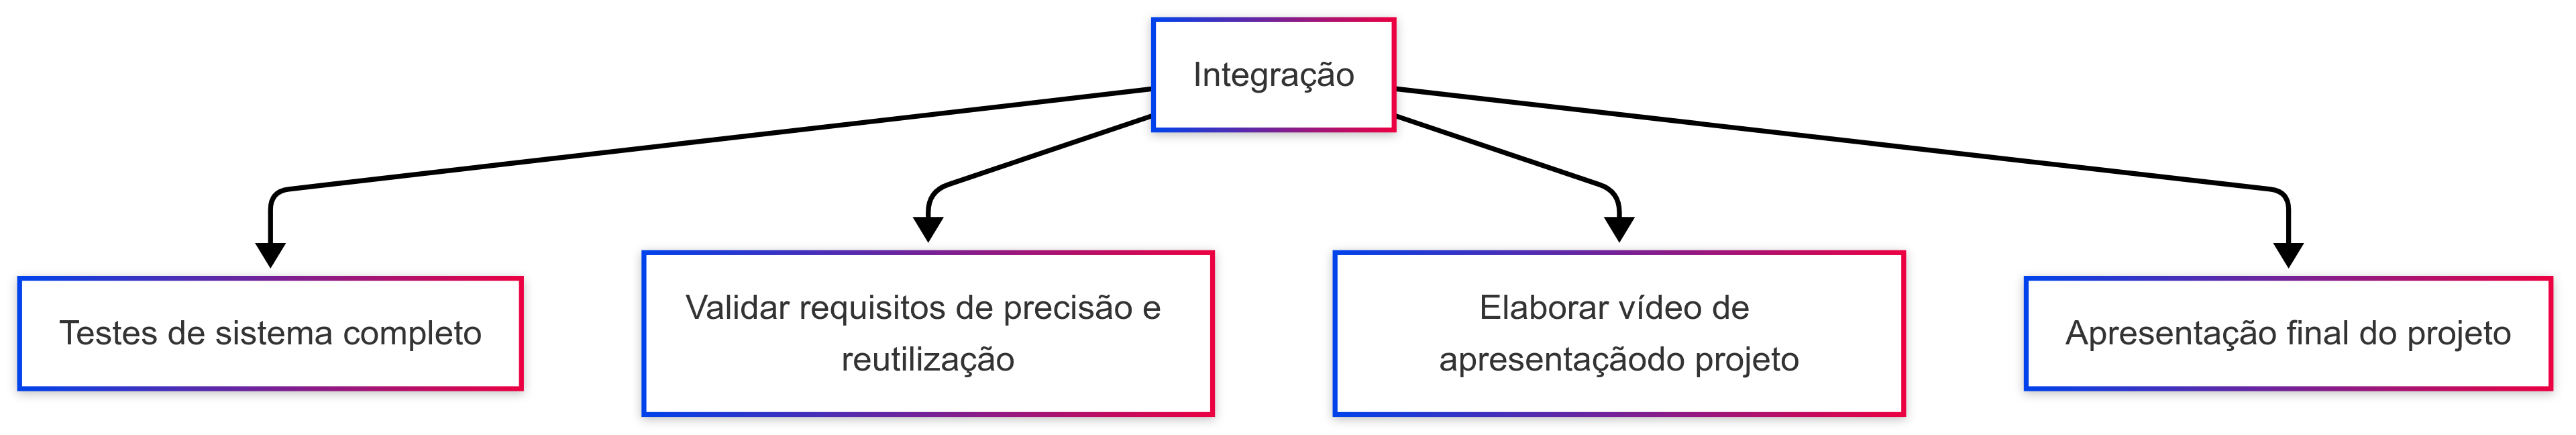
\includegraphics[width=15cm]{figuras/eap_integracao.png}
	\caption{Pacote de Trabalho 1.6 – Integração}
	\label{fig_eap_integracao}  
\end{figure}